% ****** Start of file apssamp.tex ******
%
%   This file is part of the APS files in the REVTeX 4.1 distribution.
%   Version 4.1r of REVTeX, August 2010
%
%   Copyright (c) 2009, 2010 The American Physical Society.
%
%   See the REVTeX 4 README file for restrictions and more information.
%
% TeX'ing this file requires that you have AMS-LaTeX 2.0 installed
% as well as the rest of the prerequisites for REVTeX 4.1
%
% See the REVTeX 4 README file
% It also requires running BibTeX. The commands are as follows:
%
%  1)  latex apssamp.tex
%  2)  bibtex apssamp
%  3)  latex apssamp.tex
%  4)  latex apssamp.tex
%
\documentclass[%
 reprint,
%superscriptaddress,
%groupedaddress,
%unsortedaddress,
%runinaddress,
%frontmatterverbose, 
%preprint,
%showpacs,preprintnumbers,
%nofootinbib,
%nobibnotes,
%bibnotes,
 amsmath,amssymb,
 aps,
%pra,
%prb,
%rmp,
%prstab,
%prstper,
floatfix,
]{revtex4-1}

\makeatletter
\def\Dated@name{Fecha: }%
\def\andname{y}
\makeatother

\setlength{\parskip}{3pt}

\usepackage{color}
\usepackage{lipsum}
\usepackage[utf8]{inputenc}
\usepackage[spanish, es-tabla, es-nodecimaldot]{babel}
\usepackage{graphicx}% Include figure files
\usepackage{dcolumn}% Align table columns on decimal point
\usepackage{bm}% bold math
\usepackage{hyperref}% add hypertext capabilities
%\usepackage[mathlines]{lineno}% Enable numbering of text and display math
%\linenumbers\relax % Commence numbering lines
%\renewcommand{\date}[1]{(Fecha: #1)}

%\usepackage[showframe,%Uncomment any one of the following lines to test 
%%scale=0.7, marginratio={1:1, 2:3}, ignoreall,% default settings
%%text={7in,10in},centering,
%%margin=1.5in,
%%total={6.5in,8.75in}, top=1.2in, left=0.9in, includefoot,
%%height=10in,a5paper,hmargin={3cm,0.8in},
%]{geometry}
\usepackage{multirow}
\usepackage{listings}
\newcommand{\tas}{$\text{TaS}_2$}
\newcommand{\christoffel}[3]{\Gamma^{#1}_{#2 #3}}

\begin{document}

%\preprint{APS/123-QED}

\title{Intoducción a la relatividad numérica y una aplicación \\
\small{Proyecto}}% Force line breaks with \\

\author{Nicolás Maldonado - 201423809}%
\affiliation{%
 Universidad de los Andes, Departamento de Física \\
 Relatividad General y Cosmología - FISI3090
}%

\date{\today}% It is always \today, today,
             %  but any date may be explicitly specified

\begin{abstract}

\end{abstract}

\maketitle

%\tableofcontents

\section{Introducción}

La relatividad numérica, o NR por sus siglas en inglés, es una herramienta de gran utilidad para resolver las ecuaciones de Einstein:%

\begin{equation}\label{eq:einstein}%
    G_{\mu \nu} = 8\pi T_{\mu \nu}%
\end{equation}%

En la expresión anterior se encuentran codificadas múltiples ecuaciones diferenciales parciales, si bien éstas deberían ser 16 en un espacio de dimensión 3+1, cada tensor involucrado tiene solo 10 componentes independientes. Luego, y con ayuda de las identidades de Bianchi, estas diez ecuaciones se reducen a solo seis ecuaciones independientes. Sin embargo, aún después de haberse reducido el problema a solo 6 ecuaciones, la complejidad que ocultan las ecuaciones de Einstein siguen haciendo que encontrar soluciones para las mismas sea una tarea complicada y delicada.
En (\ref{eq:einstein}), el tensor de Einstein, $G_{\mu \nu}$, resulta ser equivalente a $R_{\mu \nu}-\frac{1}{2}g_{\mu \nu}$, donde $R_{\mu \nu}$ es el tensor de Ricci, $R$ es el escalar de Ricci --la traza del tensor de Ricci--, y $g_{\mu\nu}$ es el tensor métrico. Como resultado, (\ref{eq:einstein}) puede reescribirse como:

\begin{equation}\label{eq:einstein2}%
    R_{\mu \nu} - \frac{1}{2}Rg_{\mu \nu} = 8\pi T_{\mu \nu}
\end{equation}%

Ahora, el tensor de Ricci $R_{\mu \nu}$ es la contracción 1-3 del tensor de Riemman, $R^\mu_{\hspace{5pt} \nu \rho \sigma}$, i.e. $R_{\mu \nu} = R^\lambda_{\hspace{5pt} \mu \lambda \nu}$, el cual a su vez se define a partir de los símbolos de Christoffel, $\christoffel{\lambda}{\mu}{\nu}$, y como consecuencia el tensor de Ricci puede definirse como:

\begin{equation}%
    R_{\mu \nu} = \partial_\lambda \christoffel{\lambda}{\nu}{\mu} - \partial_\nu \christoffel{\lambda}{\lambda}{\mu} + \christoffel{\lambda}{\lambda}{\sigma}\christoffel{\sigma}{\nu}{\mu} -\christoffel{\lambda}{\nu}{\sigma}\christoffel{\sigma}{\lambda}{\mu}
\end{equation}%

Ahora, todo esto puede incluirse en (\ref{eq:einstein2}), y puede reescribirse como:

\begin{equation}
    \partial_\lambda \christoffel{\lambda}{\nu}{\mu} - \partial_\nu \christoffel{\lambda}{\lambda}{\mu} + \christoffel{\lambda}{\lambda}{\sigma}\christoffel{\sigma}{\nu}{\mu} -\christoffel{\lambda}{\nu}{\sigma}\christoffel{\sigma}{\lambda}{\mu} - \frac{1}{2}Rg_{\mu \nu} = 8\pi T_{\mu \nu}
\end{equation}

Finalmente, los símbolos de Christoffel se pueden expandir en términos de derivadas parciales de la métrica:

\begin{equation}%
    \christoffel{\sigma}{\mu}{\nu} = \frac{1}{2}g^{\sigma \rho}\left(\partial_\mu g_{\rho \nu} + \partial_\nu g_{\rho \mu} -\partial_\rho g_{\mu \nu} \right)
\end{equation}%

Con esto ya se hace evidente que intentar resolver las ecuaciones de Einstein requiere un trabajo formidable en álgebra y cálculo. Si se quisieran escribir las diez ecuaciones codificadas por (\ref{eq:einstein}), sería necesario utilizar alrededor de cien páginas \cite{SimulatingeXtremeSpacetimesWhyRelativity}. En algunos casos especiales las ecuaciones de Einstein se pueden resolver analíticamente con papel y lápiz, pero en la mayoría de las situaciones esta tarea resulta imposible. Por lo tanto, es de gran interés buscar métodos numéricos que permitan la solución de las ecuaciones de Einstein.

De este interés emerge la relatividad numérica, la cual tiene como propósito buscar soluciones a las ecuaciones de Einstein en los casos más complejos, tales como el estudio de estrellas binarias compactas \cite{Baumgarte2003NumericalBinaries}, las colisiones de black holes y las ondas gravitacionales asociadas a estas \cite{Centrella2010Black-holeRelativity, Nakamura1993GravitationalRelativity}, entre otros \cite{Cardoso2015ExploringRelativity, Lehner2001NumericalReview, Lehner2014SummaryApplications, Shibata2004StatusRelativity, Piran1981PROBLEMSRELATIVITY}. Además de permitir la realización de cálculos en los casos de diversas dimensiones, desde dimensión 1 \cite{Arbona1999DealingRelativity, Gourgoulhon19921DCollapse} y 2 \cite{Font1993NumericalRelativity}, pasando por la estándar 3+1 \cite{Alcubierre2008IntroductionRelativity, Brugmann2000NumericalDimensions}, y más allá \cite{Witek2013NumericalSpace-times}.

En este proyecto se propone explorar los conceptos y técnicas más importantes de la relatividad numérica, así como ejecutar cálculos computacionales para resolver las ecuaciones de Einstein numéricamente en un caso particular.

\section{Marco teórico}

Para este proyecto es necesario profundizar en los diversos métodos numéricos y el software disponibles para solucionar problemas de relatividad general. Por otra parte, este proyecto pretende estudiar la trayectoria de un fotón en la proximidad de un black hole, por lo que es pertinente exponer el tratamiento relativista requerido para explicar dicho fenómeno.

\subsection{Métodos numéricos, álgebra computacional, y CAS}

Cuando se habla de relatividad numérica, por supuesto, se habla de métodos en el área del análisis numérico aplicados a problemas de la relatividad general. Debido a la dificultad de las ecuaciones que aparecen en la relatividad, como ya se mencionó anteriormente, esto en general implica métodos computacionales.

El álgebra computacional, también llamado cálculo simbólico o cálculo algebraico, se refiere al desarrollo de software y algoritmos para la manipulación de expresiones y objetos matemáticos de diversa índole, y frecuentemente de manera simbólica, tal y como los manipularía manualmente un matemático o científico, y en contraste a como tradicionalmente un computador solo es capaz de realizar manipulaciones matemáticas que contengan números explícitos. Gran parte de esta disciplina, desde la segunda mitad del siglo XX, ha sido el desarrollo de los llamados sistemas de álgebra computacional, o CAS por sus siglas en inglés, software matemático que permite la manipulación deseada para posibilitar el trabajo computacional en temas matemáticos y científicos de manera abstracta. Son muchos los CAS que se han desarrollado, algunos de ellos con propósitos muy específicos y otros más generales, de los cuales puede elegirse el más conveniente para el trabajo a realizar.

Así pues, resulta natural que en la relatividad numérica, en la que se quiere estudiar espacio-tiempos cuya forma exacta no se conoce, y que por lo tanto requieren un tratamiento abstracto y simbólico, la herramienta computacional más usada sea algún CAS, especialmente aquellos que permiten manipulación de tensores y PDEs, pues este es el lenguaje matemático de la relatividad general \cite{Guzman2007IntroductionExamples, Heinicke2002ComputerGravity, MacCallum2018ComputerResearch, MacCallum2002ComputerRelativity}.

Algunos de los CAS más usados y encontrados a lo largo de la literatura son Wolfram Mathematica\textsuperscript{\textregistered} \cite{Baumann2005Mathematica2, HartleGravity:Relativity, Hrabovsky2014GeneralMathematica, Koberlein2013AstrophysicsSupport, Woszczyna2016SYMBOLICAPPROACH, Zimmerman2001GeneralMathematica}, SageMath \cite{Birkandan2019SymbolicSystems, Vankov2016GeneralTest}, y el módulo GraviPy para Python\textsuperscript{\textregistered} \cite{Birkandan2019SymbolicSystems, Woszczyna2016SYMBOLICAPPROACH}.

\subsection{Trayectoria de un fotón próximo a un black hole}

Además de la solución de problemas en relatividad general, la relatividad numérica también permite esclarecer ciertos temas en astrofísica y cosmología \cite{Barack2019BlackRoadmap, Lehner2014NumericalAstrophysics, Seidel1999NumericalAstrophysics}. Un problema simple en relatividad general, con aplicaciones en astrofísica, y que puede ser resuelto mediante relatividad numérica, es el de la trayectoria de un fotón próximo a un black hole. Si bien el tema de los black holes siempre ha sido de gran importancia para la relatividad general, siendo esta teoría la que primero los predijo, con la aparición de los primeros resultados del Event Horizon Telescope en Abril del presente año \cite{Akiyama2019FirstHole, Akiyama2019FirstHoleb} ha habido un creciente interés en este tema y en particular en el entendimiento de qué es exactamente lo que se aprecia en la imagen \cite{Akiyama2019FirstRing}. Dicho de otra manera, se quiere entender la trayectoria que siguieron los fotones que finalmente llegaron al arreglo de telescopios y dieron lugar a las imágenes publicadas, y esta trayectoria básicamente fue dictada por el black hole cuya imagen se estaba intentando capturar.
Así pues, se pueden aplicar métodos numéricos al estudio de este problema particular, teniendo en cuenta lo que se sabe de los black holes de la relatividad general y planteando el problema de dinámica que aquí surge, y llegando finalmente a soluciones para las trayectorias de los fotones alrededor del black hole, pudiendo esclarecerse así el origen de lo que se observa en las imágenes de M87 \cite{Nolte2019OrbitingHole}.

\section{Cálculos Numéricos}

\subsection{Esfera de fotones}

Una esfera de fotones es una región del espacio donde la gravedad es tan fuerte que los fotones se ven forzados a moverse en órbitas. El radio de una esfera de fotones, que además resulta ser el radio más pequeño que admite órbitas estables, puede ser calculado a partir de una métrica apropiada. En este caso partimos de la métrica de Schwarzschild

\begin{align}
    ds^2 = \left(1 - \frac{r_S}{r}\right) dt^2 - \left(1 - \frac{r_S}{r}\right)^{-1} dr^2 - r^2 d\Omega^2
\end{align}

introducimos en Mathematica\textsuperscript{\textregistered} el número de dimensiones, las coordenadas a usar, y la métrica en forma matricial. Se procede además a calcular la métrica inversa.

\onecolumngrid
\vspace{12pt}
\hrule
\begin{lstlisting}[language=Mathematica]
    n = 4;

    coord = {r, \[Theta], \[Phi], t};
    
    metric = ({{-(1 - \[ScriptR]/r)^-1, 0, 0, 0},
        {0, -r^2, 0, 0},
        {0, 0, -r^2 Sin[\[Theta]]^2, 0},
        {0, 0, 0, 1 - \[ScriptR]/r}});
    
    inversemetric = Simplify[Inverse[metric]];
\end{lstlisting}
\hrule
\vspace{12pt}
\twocolumngrid

Enseguida se usan estas matrices para calcular directamente los símbolos de Christoffel y mostrarlos.

\onecolumngrid
\vspace{32pt}
\hrule
\begin{lstlisting}[language=Mathematica]
christoffel = 
  Simplify[Table[
    1/2 Sum[inversemetric[[i, s]] (D[metric[[s, j]], coord[[k]]] + 
         D[metric[[s, k]], coord[[j]]] - 
         D[metric[[j, k]], coord[[s]]]), {s, 1, n}], {i, 1, n}, {j, 1,
      n}, {k, 1, n}]];

listchristoffel = 
  Table[If[UnsameQ[christoffel[[i, j, k]], 
     0], {ToString[\[CapitalGamma][i, j, k]], "=", 
     christoffel[[i, j, k]]}], {i, 1, n}, {j, 1, n}, {k, 1, n}];
     
TableForm[Partition[DeleteCases[Flatten[listchristoffel], Null], 3], 
 TableSpacing -> {2, 2}]
\end{lstlisting}
\hrule
\vspace{12pt}
\twocolumngrid

Que inmediatamente extrae

\begin{align}
    \begin{split}
    & \Gamma^t_{tr} = \tfrac{r_S}{2r^2 - 2r_Sr} \quad \Gamma^r_{tt} = \tfrac{(r-r_S)r_S}{2r^3} \quad \Gamma^r_{rr} = -\tfrac{r_S}{2r^2 - 2r_Sr}\\
    & \Gamma^r_{\theta\theta} = -r+r_S \quad \Gamma^r_{\phi\phi} = -(r-r_S)\sin^2{\theta} \quad \Gamma^\theta_{r\theta} = -\tfrac{1}{r}\\
    & \Gamma^\theta_{\phi\phi} = -\cos{\theta}\sin{\theta} \quad \Gamma^\phi_{r\phi} = \tfrac{1}{r} \quad \Gamma^\phi{\theta\phi} = \cot{\theta}
    \end{split}
\end{align}

las nueve componentes independientes distintas de 0. Ahora pues, se usan estas conexiones para calcular las ecuaciones geodésicas para cada componente de la 4-velocidad, $U^\mu$.

\onecolumngrid
\vspace{12pt}
\hrule
\begin{lstlisting}[language=Mathematica]
geodesic = 
  Simplify[Table[-Sum[
      christoffel[[i, j, k]] u[j] u[k], {j, 1, n}, {k, 1, n}], {i, 1, 
     n}]];
     
listgeodesic = 
  Table[{"\!\(\*FractionBox[\(d\), \(d\[Tau]\)]\)" ToString[u[i]], 
    "=", geodesic[[i]]}, {i, 1, n}];

TableForm[listgeodesic, TableSpacing -> {2, 2}]
\end{lstlisting}
\hrule
\vspace{12pt}
\twocolumngrid

Y se llega a las siguientes ecuaciones

\begin{align}
    \tfrac{d}{d\tau}U^t &= - \tfrac{(r-r_S)r_S}{2r^3}(U^t)^2 -\tfrac{r_S}{r^2-r_Sr}U^tU^r \label{Ut}\\
    \tfrac{d}{d\tau}U^r &= {\scriptstyle(r-r_S)}\left[ \tfrac{r_S}{2r(r-r_S)^2}(U^r)^2 + (U^\theta)^2 + \sin^2{\theta}(U^\phi)^2\right] \label{Ur}\\
    \tfrac{d}{d\tau}U^\theta &= -\tfrac{2}{r}U^rU^\theta + \cos{\theta}\sin{\theta}(U^\phi)^2 \label{Uth}\\
    \tfrac{d}{d\tau}U^\phi &= -\tfrac{2}{r}U^rU^\phi -2\cot{\theta}U^\theta U^\phi \label{Uph}
\end{align}

luego usando (\ref{Ur}), y considernado que $\frac{dr}{d\tau},\frac{d^2r}{d\tau^2},\frac{d\theta}{d\tau} = 0$ se llega a la relación

\begin{align}\label{geo}
    \left(\frac{d\phi}{dt}\right)^2 = \frac{r_S}{2r^3\sin^2{\theta}}
\end{align}

Por otra parte se tiene que para fotones el intervalo espacio-temporal es de tipo nulo, i.e., $ds^2 = 0$, y haciendo la escogencia adecuada de coordenadas tales que $dr = 0$ y $d\theta = 0$, se puede manipular la métrica de tal manera que se pueda escribir

\begin{align}\label{met}
    \frac{d\phi}{dt} = \frac{1}{r\sin{\theta}}\sqrt{1-\frac{r_S}{r}}
\end{align}

Finalmente se comparan directamente (\ref{geo}) y (\ref{met}) y se llega al radio de la esfera de fotones en términos del radio de Schwarzschild, $r_S$,

\begin{align}
    r = \frac{3}{2}r_S
\end{align}

\subsection{Trayectorias de fotones}

Ahora se quieren calcular las trayectorias de fotones en la cercanía del black hole, para ello se usan (\ref{Ut}) y (\ref{Ur}) para hallar la velocidad

\begin{align}
    \frac{dr}{dt} = \frac{r-r_S}{r} = c(r)
\end{align}

y de manera análoga a como se tiene el índice de refracción para un material, se calcula el "índice de refracción" gravitacional, $n(r) = c/c(r)$, en este caso como se tienen unidades con $c=1$ se tiene directamente

\begin{align}
    n(r) \equiv \frac{1}{c(r)} = \frac{1}{1-\frac{r_S}{r}}
\end{align}

Este "índice de refracción" resulta importante para introducirlo en la ecuación de Eikonal

\begin{align}
    \frac{d}{d\tau}\left(n\frac{dx^\nu}{d\tau}\right) = \partial_\nu n
\end{align}

de donde sale el sistema de ecuaciones diferenciales ordinarias que se resolverá a continuación numéricamente

\begin{align}\label{sys}
    \begin{split}
    \frac{dx}{d\tau} &= \frac{1}{n}\dot{x}\\
    \frac{dy}{d\tau} &= \frac{1}{n}\dot{y}\\
    \frac{d\dot{x}}{d\tau} &= \partial_xn\\
    \frac{d\dot{y}}{d\tau} &= \partial_yn
    \end{split}
\end{align}

El sistema (\ref{sys}) se introduce en la función \texttt{NDSolve} de Mathematica\textsuperscript{\textregistered} con 36 distintas condiciones iniciales (en realidad la única condición inicial que cambia es la posición en $y$) y se genera una gráfica con todas las trayectorias, además de la esfera de fotones y el disco al interior del radio de Schwarzschild.

\onecolumngrid
\vspace{12pt}
\hrule
\begin{lstlisting}[language=Mathematica]
xsoln = ConstantArray[0, 36];
ysoln = ConstantArray[0, 36];
For[i = -5, i < 31, 
 i++, {n[t_] = Sqrt[x[t]^2 + y[t]^2]/(-10 + Sqrt[x[t]^2 + y[t]^2]), 
  nx[t_] = -((x[t] 10)/(
    Sqrt[x[t]^2 + y[t]^2] (Sqrt[x[t]^2 + y[t]^2] - 10)^2)), 
  ny[t_] = -((y[t] 10)/(
    Sqrt[x[t]^2 + y[t]^2] (Sqrt[x[t]^2 + y[t]^2] - 10)^2)), 
  sol = NDSolve[{x'[t] == vx[t]/n[t], y'[t] == vy[t]/n[t], 
     vx'[t] == nx[t], vy'[t] == ny[t], x[0] == -100, 
     y[0] == -2.245 + 4 i, vx[0] == n[0], vy[0] == 0}, {x[t], y[t], 
     vx[t], vy[t]}, {t, 0, 2000}], xsoln[[i + 6]] = sol[[1, 1]], 
  ysoln[[i + 6]] = sol[[1, 2]]}]
  
color = {RGBColor[0.27, 0.45, 0.6], RGBColor[0.95, 0.58, 0.29], 
   RGBColor[0.44, 0.69, 0.38], RGBColor[0.8, 0.36, 0.35], 
   RGBColor[0.61, 0.49, 0.75], RGBColor[0.6, 0.46, 0.42], 
   RGBColor[0.86, 0.59, 0.79], RGBColor[0.57, 0.57, 0.57], 
   RGBColor[0.78, 0.78, 0.38], RGBColor[0.42, 0.78, 0.84]};
plots = ConstantArray[0, 36]
For[i = 1, i < 37, i++, 
 plots[[i]] = 
  ParametricPlot[{x[t] /. xsoln[[i]], y[t] /. ysoln[[i]]}, {t, 0, 
    2000}, PlotRange -> {{-100, 100}, {-100, 100}}, Frame -> True, 
   Axes -> False, PlotStyle -> color[[Mod[i, 10, 1]]]]]
   
schwarzschild = RegionPlot[Disk[{0, 0}, 10], PlotStyle -> Black];
sphere = RegionPlot[Circle[{0, 0}, 15], PlotStyle -> Black];
Show[plots, schwarzschild, sphere]
\end{lstlisting}
\hrule
\vspace{24pt}

\begin{figure}
    \centering
    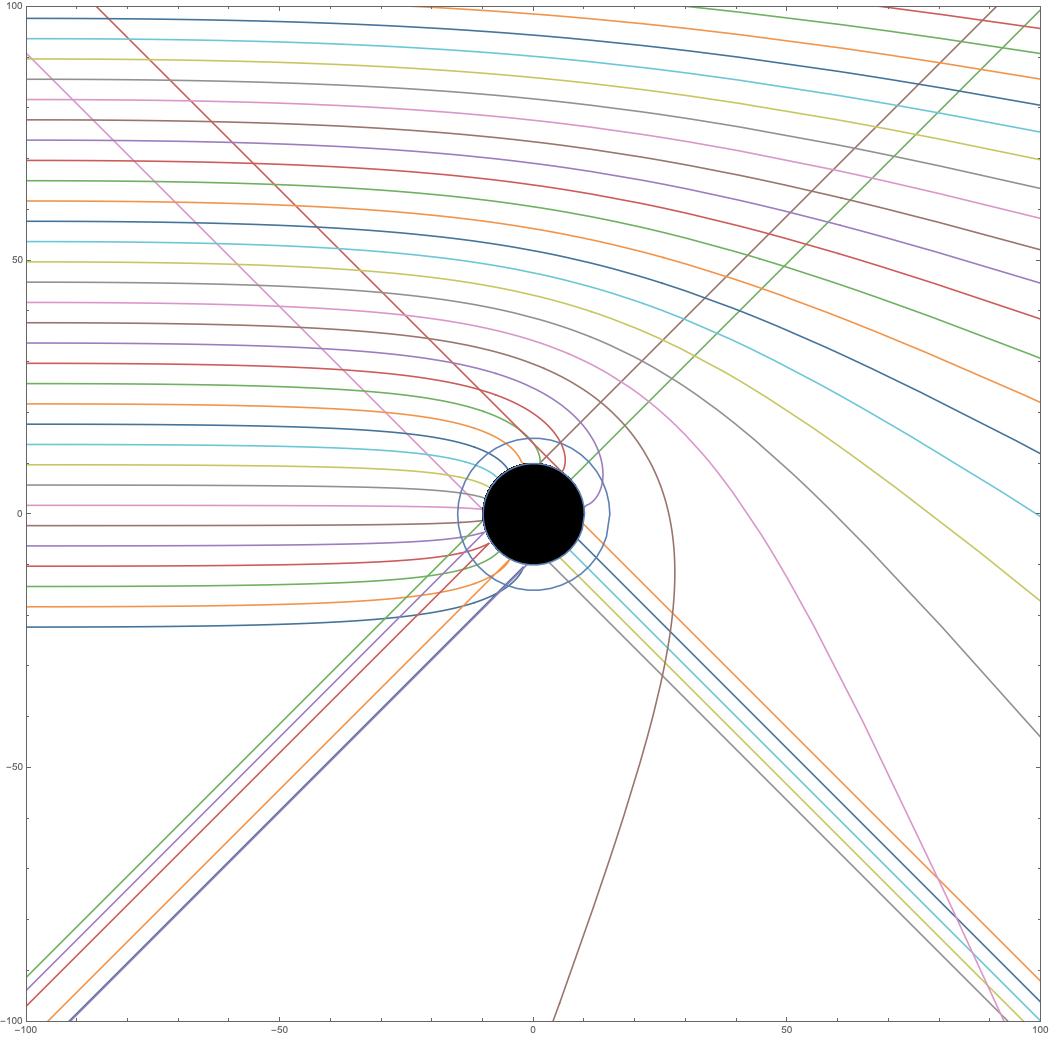
\includegraphics[width=\textwidth]{photons.png}
    \caption{Gráfica generada por Mathematica\textsuperscript{\textregistered} para las trayectorias de 36 fotones sujetos a distintas condiciones iniciales, la esfera de fotones, y el disco al interior del radio de Schwarzschild.}
    \label{fig:photons}
\end{figure}
\twocolumngrid

Esta gráfica puede compararse directamente con la producida usando Python en \cite{Nolte2019OrbitingHole}. Es claro que aunque las trayectorias en general fueron calculadas correctamente, para aquellas trayectorias que inciden en $y < \frac{3}{2}r_S$ ésta se daña después de este punto, es claro entonces que hace falta alguna corrección en el proceso que se asegure de que se encontrarán soluciones válidas también en esta región.

\section{Conclusión}

Se logró consultar bibliografía que resaltara los aspectos más importantes de la relatividad numérica, así como las herramientas y los métodos que se usan en ella, y el tipo de problemas que podrían resolverse por medio de éstos. Se logró además realizar algunos cálculos simples para un caso específico, aunque como ya se mencionó faltó alguna corrección para una cierta región del espacio (donde la trayectoria pasa por un $r < \frac{3}{2}r_S$). No obstante, se logró comprobar por medio de estos cálculos el poder de los métodos numéricos en relatividad general. Las trayectorias encontradas además dan cuenta de lo que se observa en las imágenes de M87 publicadas más temprano este año \cite{Akiyama2019FirstRing} (ver \cite{Nolte2019OrbitingHole}).

Como trabajo futuro se propone estudiar trayectorias análogas a estas partiendo de la solución de Kerr para black holes con momento angular.

\bibliography{references.bib}

\end{document}